\chapter{Methodology}

This chapter describes all the required steps to achieve a functional deep neural network to participate at the ActivityNet Challenge. For this challenge there was no baseline because video tasks have not been faced on the group I did this project, so was required to face the challenge from scratch.

% AMAIA: Again I think that it is assumed that you did all the work explained in this project.

\section{Objective}

The aim of this project is to design and train a deep neural network to classify and temporally localize activities in videos. The network is designed to exploit temporal information by using Recurrent Neural Networks (RNNs). The network is trained using 3D convolutional features from short video clips (16 frames each), which are fed to the network sequentially. The network is expected to output a label for each short video clip, preserving temporal consistency between close predictions in the output sequence. The design of the network enables both activity classification and detection capabilities using simple post-processing techniques on its output.

% AMAIA: I have changed this a bit. I think that all claims & comparison with other works should be done in the state of the art, results and conclusion sections. Here you should just explain your work.

%In order to get that, the proposal is, once the features have been extracted with the C3D, predict with a RNN a sequence of activities that might be happening for every 16-frame clip. So as the output of the Neural Network, is expected to have a sequence each item giving the activity happening at each video clip as input. This approach offers more advantages that others being able to classify the whole video and even localize along the video sequence them multiple activities happening and their temporal localization.

\section{ActivityNet Dataset}

The ActivityNet Dataset\cite{caba2015activitynet} is \textit{A Large-Scale Video Benchmark for
Human Activity Understanding}. This dataset (on its version 1.3, the one used for the challenge), contains 19,994 videos with different 200 activities labeled, representing a wide range of human activities. 

\begin{figure}[t]
\begin{center}
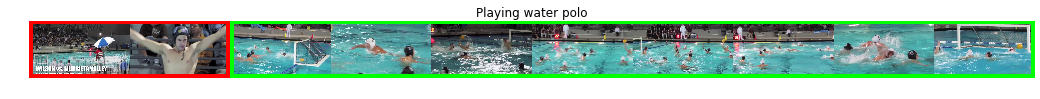
\includegraphics[width=1\linewidth]{img/methodology/activitynet_examples/activitynet_example_1}
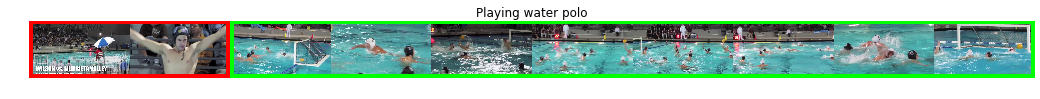
\includegraphics[width=1\linewidth]{img/methodology/activitynet_examples/activitynet_example_2}
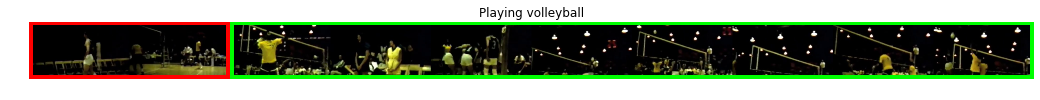
\includegraphics[width=1\linewidth]{img/methodology/activitynet_examples/activitynet_example_3}
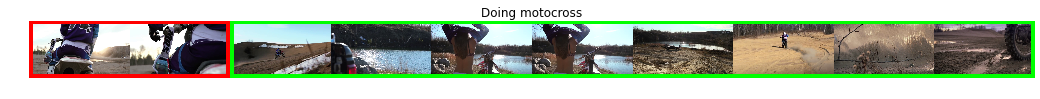
\includegraphics[width=1\linewidth]{img/methodology/activitynet_examples/activitynet_example_4}
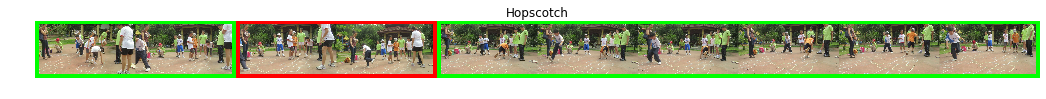
\includegraphics[width=1\linewidth]{img/methodology/activitynet_examples/activitynet_example_5}
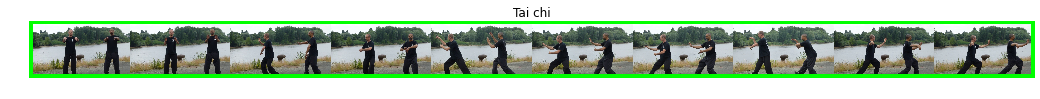
\includegraphics[width=1\linewidth]{img/methodology/activitynet_examples/activitynet_example_6}
\end{center}
\caption{Sample of videos from the ActivityNet Dataset}
\label{fig:dataset_example}
\end{figure}
% AMAIA: I think this section is asking for a figure with some examples of the dataset :). Maybe they have a figure like this in the website or their paper already? ALBERTO: DONE

In total there are 660 hours of video and the subsets are split in the following way: 50\% training set, 25\% validation set and 25\% testing set. Each video of the dataset is annotated with a single activity along with the annotation of all temporal locations in which the activity occurs. On the Figure~\ref{fig:dataset_example} there is examples of videos of different activities and its temporal annotations.

The dataset was provided as a description file, which the URL of the video was provided and also the ground truth annotations for the training and validation subset as a set of starting time, ending time and the activity happening between the given interval. In addition more information was given such as the original video resolution and the duration.

Because all the video from this dataset are hosted on \textit{YouTube}, only the links for the video are provided because of copyright issues. For this reason, the first task was to download all the videos given their URLs. This was done using a library called \textit{youtube-dl}, which allows to download videos from that YouTube using Python. Some issues arose during the acquisition of the dataset, such as videos being removed by their owners, or being blocked due to localization restrictions. In those cases, videos could not be downloaded and therefore were not used in the experiments. The total size of the used dataset was of 19,811 videos.

% AMAIA: I changed some of the text above to be less informal in general... but you should try to do it from this point on.

Once the videos from the dataset were downloaded, the number of frames of each video was extracted to be able in the future to convert from seconds to frames in the temporal domain. 

% AMAIA: I don't understand what you mean in the above text. I guess you want to say that all frames from all videos are used ( no subsampling)? The resolution part I don't get. In any case, this does not belong in this section. You should explain this when you talk about feature extraction.
% ALBERTO: ok done

In addition to this, some stats were computed. Such as the whole number of frames from all the videos in the dataset which is 65.6 million frames. Also, the length in minutes of each activity at the dataset was plot on Figure~\ref{fig:dataset_stats} to have an idea about the activities duration. As it can be observed, not all the activities have the same duration along the dataset, varying from 40 minutes as the total activity appearance to 3.5 hours for the longest activity. In total, over all the dataset there are 313 hours of activities which need to be detected and localized.

\begin{figure}[ht]
\begin{center}
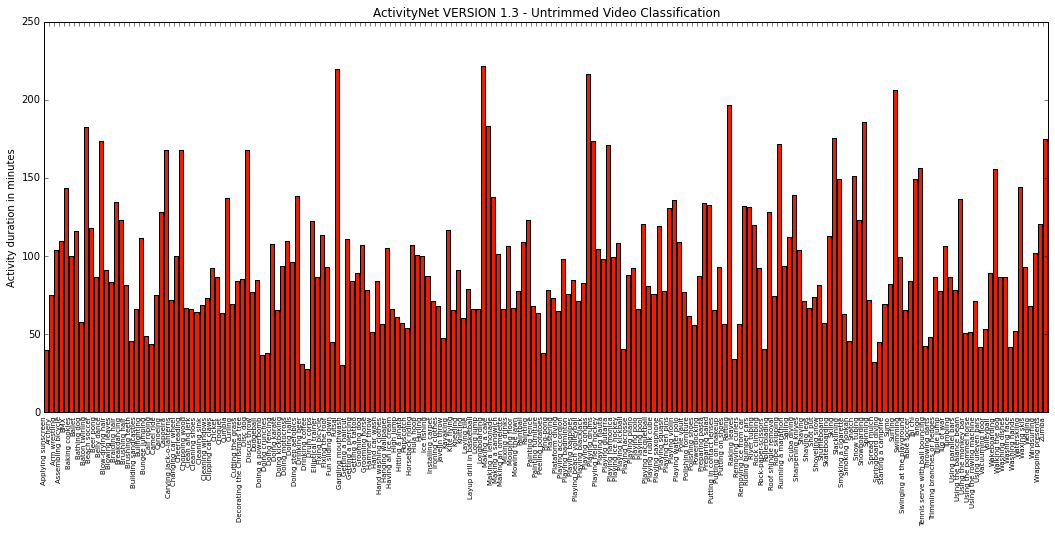
\includegraphics[width=1\linewidth]{img/methodology/dataset_stats}
\end{center}
\caption{Activity duration in minutes for each activity in the dataset}
\label{fig:dataset_stats}
\end{figure}

\section{Extracting Video Features Using C3D}

The C3D network\cite{tran2014learning} was chosen as a feature extractor, due to its success in other works in the literature \cite{baccouche2011sequential,tran2015deep,tran2014learning,shoutemporal}. This network is composed of 8 convolutional layers, plus 5 pooling layers, 2 fully-connected layers and a Softmax output at the end. The convolutional layers have $3 \times 3 \times 3$\footnote{For notation, the dimension ordering is $d \times k \times k$ where $d$ is temporal dimension and $k$ is spatial dimension} kernels and stride 1 while at the same time the pooling layers compute the maximum at every kernel size of $2 \times 2 \times 2$ (except from the first pooling layer which has a $1 \times 2 \times 2$ kernel size). The two full-connected layers (\textit{fc6} and \textit{fc7}) have both 4096 neurons while the Softmax output has 200 outputs as the number of classes of the Sports1M Dataset. Figure~\ref{fig:c3d_architecture} shows a representation of the C3D architecture, including the number of kernels or neurons of each convolutional layer and fully-connected layer respectively.

\begin{figure}[H]
\begin{center}
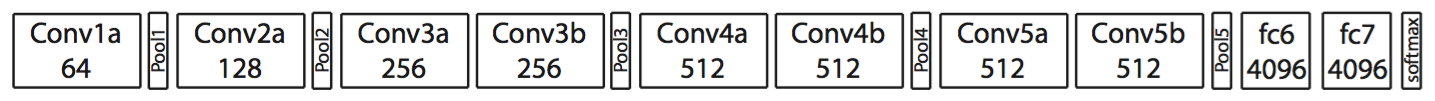
\includegraphics[width=1\linewidth]{img/methodology/c3d_architecture}
\end{center}
\caption{The C3D Architecture}
\label{fig:c3d_architecture}
\end{figure}

The input of the network are clips of videos of 112x112 frames width and height and 16 frames of temporal depth. It was decided to extract the video features at the full-connected layer \textit{fc6} because being the first after the convolutional features. It has been commonly used the values of the convolutional layers or after them as image and video feature extractors.

The original paper proposing and studying 3D convolutions applied to videos, also give code to reproduce it. The code given was based on a version of \textit{Caffe}\cite{jia2014caffe} dated in 2014. Because the code to use 3D convolutions did not support last features (such as Recurrent Neural Networks) and did not work with the \textit{Python} environment used for this project, the model trained with C3D and the Sports1M\cite{KarpathyCVPR14} dataset was ported to \textit{Keras}\footnote{All the process has been open sourced and can be found in: \url{https://gist.github.com/albertomontesg/d8b21a179c1e6cca0480ebdf292c34d2}}.

% AMAIA. Comments for the above text:
% 1. The sentence explaining what keras is should go someplace else (maybe in the requirements section ?) ALBERTO: Put on requirements.
% 2. I thought we did not use caffe because it does not support RNNs (at least not the 'vanilla' version right?) RIGHT

%%%% KEEP going here



At the time to run the C3D model on the model ported to \textit{Keras}, some small changes were applied Keras' source code\footnote{The fork of \textit{Keras} used can be found in: \url{https://github.com/albertomontesg/keras/tree/develop}}, involving the implementation of the 3D convolution and 3D pooling operations. Once this was fixed, all the videos were forwarded through the C3D model, and the features from the first fully connected layer \textit{fc6} were extracted. This process was done using 2 GPUs in parallel for feature extraction, and multiple CPU cores fetching all the videos from disk. The usage of 2 GPUs in parallel reduced the computational time expected for this task from 1 week to 2 days.

% AMAIA: I think that before the above paragraph you should say that you use 16-frame clips, and that you extract a fc6 for each of them. ALBERTO: I think that now done. 

In the process of fetching the videos from disk, the \textit{OpenCV}\cite{opencv_library} library was used. With this software, the videos were read in chunks of 16 frames, resized to 112x112 as input frame size, remove the mean for each color channel which the original model was trained with and then forwarded through the C3D network. The values of the model at the full-connected layer fc6, a sequence of 4096-sized vectors was stored in disk for preparing it to train the Recurrent Neural Network. % AMAIA: fc6 is not the output of the model, but the features that you chose to extract. ALBERTO: Change

\section{Extracting Audio Features}

The next step after extracting the video features is to extract the features coming from the videos audio track. As has been done previously for activity detection~\cite{xu2015uts}, some audio descriptors were extracted to improve the detection and classification results. On this project, the MFCC and Spectral descriptors were decided to be used as they extract a lot of information from the videos' audio~\cite{heittola2013context}. 

Both MFCC and Spectral descriptors were extracted using specialized software: SPro~\cite{gravier2010spro} and Essentia~\cite{bogdanov2013essentia} respectively. For the MFCC descriptors, 40 values were extracted for 10ms temporal windows. Because the misalignment of scale between the features extracted for video and MFCC videos, the second ones were grouped to have the same sequence length of audio features and video features. 

In order to not loose too much information at the time to group the features, the mean and standard deviations along the temporal scale were computed so at the end 80 values were available to represent the MFCC features from the audio video's track.

On the other hand, the Spectral features were extracted to have information about the energy distribution on the frequency domain along the video so only 8 values were extracted for each videos. At the time to give the audio features at the input of the Recurrent Neural Network, for each video clip feature vector, it was concatenated the MFCC features grouped for the temporal window of the clip and then also concatenated the spectral features of the whole video the clip belong. 

\section{Networks Configuration}

So as to achieve the aim of this project, which is to find a good Neural Network which is capable of classify activities and detect its temporal location in videos, the Recurrent Neural Networks were decided to be used with LSTM which have been demonstrated to learn from long term correlations. The RNN had the inputs and output previously explained, and so an experimentation of the architecture was done. 

The basic architecture consist in a single layer of LSTM with 512 cells which end-up with a total of 9.5 millions parameters. From this network as a basic one, on this project there has been some experimentation trying with more deep networks with even more cells. On Figure~\ref{fig:lstm_architecture} there is represented the network architecture.

\begin{figure}[H]
\centering
\begin{subfigure}[b]{.5\textwidth}
  \centering
  \includegraphics[width=1\linewidth]{img/methodology/lstm_architecture_basic}
\end{subfigure}%
\begin{subfigure}[b]{.5\textwidth}
  \centering
  \includegraphics[width=1\linewidth]{img/methodology/lstm_architecture_deep}
\end{subfigure}
\caption{Architecture of RNN used with 512-LSTMs with one and two layers respectively.}
\label{fig:lstm_architecture}
\end{figure}

With the basic architecture was observed that the activity prediction, in some cases was very different in short periods of time, predicting between two activities or one activity and the background class. To solve this problem, another architecture proposed consist in the previous basic one, but with an additional input at the bottom which consist the previous output of the sequence. This kind of feedback, was expected to give more smooth predictions as the network is aware about which was exactly the previous activity predicted.

For this network, a new input was added to the video features which was the one-hot encoding of the previous output with an added value, which will be always zero except to the first video feature, which do not have previous output, and will be marked with a one. With this extra value, is expected that the network learn to forget its memory state because the begging of a video sequence. In the Figure~\ref{fig:lstm_architecture_feedback} can be found the architecture previously explained with feedback.

\begin{figure}[H]
\begin{center}
\includegraphics[width=0.6\linewidth]{img/methodology/lstm_architecture_feedback}
\end{center}
\caption{Architecture of the RNN network with feedback from the previous output}
\label{fig:lstm_architecture_feedback}
\end{figure}



%%%%% Talk about semisupervised training???????


\section{Data Preparation}

At training neural networks, both the input and output data are grouped in batches to perform parallel and faster computations of the learning algorithm. This batches have the same size and contains a multiple fixed length sequence of both inputs and outputs of the dataset. The length of the sequence given at each batch is called \textit{timestep} and must a value not very high as the gradient propagate along all the sequence, and if it is high, the gradient might achieve high values known as \textit{exploiting gradient}.

Since in all major video datasets, videos are not from the same length, the videos data must be carefully prepared. It is required, if the goal is learn from long sequence data, as it is the videos of the dataset, to keep the memory of the LSTM alive for long sequences. 
% AMAIA: You should add a section explaining your architecture before you start talking about how to train it ! So basically section 3.6 should come before this one. ALBERTO:DONE

% AMAIA: A friendly intro explaining that  deep nets are usually trained on batches, which contain many samples of the dataset (of the same size)and are processed in parallel. The problem you have is that videos are too long and therefore do not fit in a single batch (risk of exploding gradients as well), so you need to cut them in pieces to separate them in different batches, and also make sure that LSTM memory is preserved from batch to batch.

% REMOVED: Since all the videos on the ActivityNet Dataset are not from the same length, to train a recurrent neural network, it requires to give it a fixed length sequence. This length is called \textit{timestep} and must be a value not very high because as the gradient propagates along all the sequence, if the timestep is very high, the gradient might achieve very high values known as \textit{exploiting gradient}.

There are two main solutions to this problem. The first solution is to have the data in batches with large \textit{timestep} but it would require to clip the gradients as it is explained in \cite{pascanu2012difficulty}. The second solution is to train the Recurrent Neural Network without resetting the memory from batch to batch. With this approach, if a video sequence is longer than the \textit{timestep}, the RNN can be trained passing fragments of the videos as clips one after the other in different batches, but at the same batch position. Since the memory is not reset after each batch, the video sequence is processed smoothly. For this configuration, the different videos must be carefully set on the same batch index to exploit the \textit{Keras} functionality of stateful training for RNNs.

\begin{figure}[ht]
\begin{center}
\includegraphics[width=1\linewidth]{img/methodology/stateful_dataset}
\end{center}
\caption{Graphical representation of how the data is sorted in batches}
\label{fig:stateful_dataset}
\end{figure}

Figure~\ref{fig:stateful_dataset} depicts how the video features are organized to train the Recurrent Neural Network. The notation for the data is as follows: $\bar{X}$ is the feature vector of a 16 frame clip extracted from the C3D network, and $V_i$ the sequence of features for a single video. Note that $T_i$ is the length of the sequence of each video $i$ in number of 16-frame clips.

\begin{equation}
	\bar{X} = [x_i, x_2, \ldots, x_{4096}]
\end{equation}
\begin{equation}
	V_i = \{ \bar{X}_t \}_{t=1}^{T_i}
\end{equation}

%In order to try to fit the most possible data into the GPUs when training each batch and to get a good gradient propagation along the batch's sequence length, for all the experiments done on this project, the batch size was 256 and the timesteps 20. % AMAIA: The values of this parameters should be given in the experiments section- % ALBERTO: Completely agree

As the last step to prepare the data, the output information was computed for each 16-frame clip as follows: if the Intersection Over Union (IOU) between the temporal range of the 16-frame clip and the ground truth annotations was higher than $0.5$, the clip was cataloged as the activity of the ground truth annotation. If the IOU was lower, it was cataloged as background activity. So at the training and validation subsets, the output was encoded with the one-hot encoding, which puts a 1 at the position of the class given and 0s on the rest. This way to encode the output is the used for Softmax output layers which represent the probability of each class to be predicted as the output is between 0 and 1.

% AMAIA: The above paragraph is explaining the evaluation of the output. This does not go here, but later in the experiments section. ALBERTO: NO, this is trying to explain how is set the output for training for each of the 16-frames clips. This is the step of how I pass from a list of temporal annotations to have some 16-frame clips with a class on each.
% AMAIA: Again, the explanation of how to encode class labels as one-hot vectors should come later. ALBERTO: This is how the output data is prepared. I think that may fit better on the methodology chapter.


\section{Training}
\label{section:training}
% ALBERTO: I'm aware that there are two sections call training both in methodology and results. May I change the name of this one??

At the time to train, some parameters required to be specified, and some problems appear with them. For training a loss function was chosen, also known as objective function. For the configuration proposed, the best loss function to choose is the categorical cross entropy because the use of Softmax as output which predicts each activity probability and can be considered as a probability distribution. It is computed as follows,

\begin{equation}
	H(p,q) = - \sum_x p(x) \log(q(x))
\end{equation}

where $q$ is the predicted probability distribution and $p$ the ground truth probability distribution.

%Another important parameter to setup for training is the optimizer function. For training Recurrent Neural Networks, the best choice is to use the RMSprop\cite{dauphin2015rmsprop} with a value of $\rho$ of 0.9 and $\epsilon$ of $10^{-8}$. 
The learning rate, otherwise, have been the value that has need to be tuned. At the training, starting with high values for the learning rate, it was observed that the network did not learned and the validation loss increased instead of decreasing. On the Figure~\ref{fig:training_curves_comparison} can be seen the difference between training the same network with a different values of learning rate. Finally the best learning rate that was found to work better at the time to train is $10^{-5}$.

\begin{figure}[H]
\centering
\begin{subfigure}[b]{.5\textwidth}
  \centering
  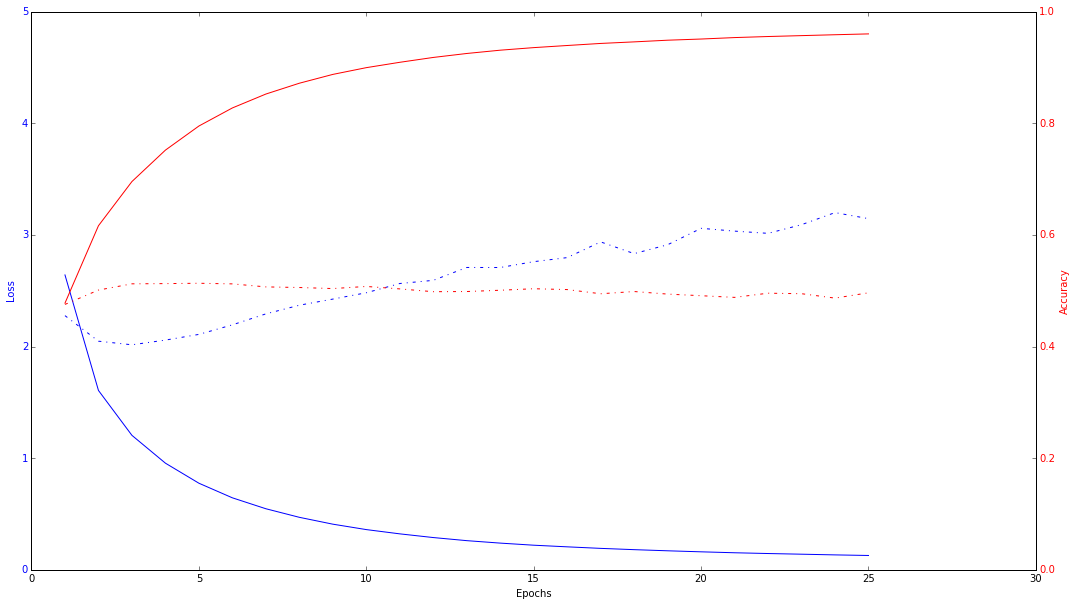
\includegraphics[width=1\linewidth]{img/methodology/training_bad}
\end{subfigure}%
\begin{subfigure}[b]{.5\textwidth}
  \centering
  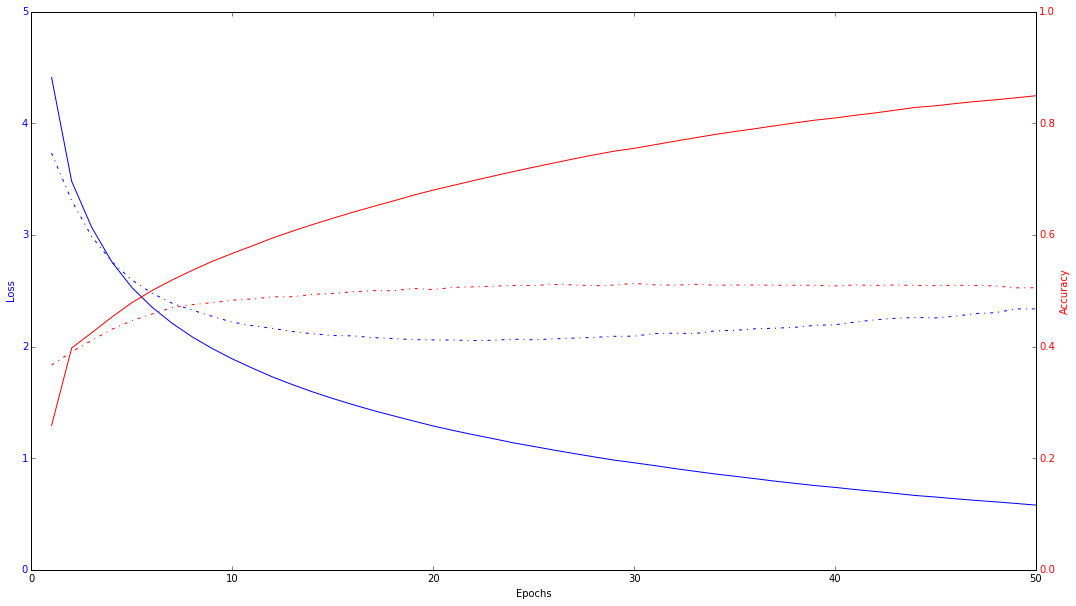
\includegraphics[width=1\linewidth]{img/methodology/training_good}
\end{subfigure}
\caption{Comparison of the learning curves. On the left with a learning of $10^{-4}$ and at the right figure with a learning rate of $10^{-5}$}
\label{fig:training_curves_comparison}
\end{figure}

In addition to find the right value for the learning rate, some other problems appear. Even with a good learning rate to learn, it was observed that the network presented some over-fitting due mostly to the high learning capacity the network has over the data. So, in order to fix that, dropout\cite{srivastava2014dropout} layers were added before and after the LSTM layers to reduce this over-fitting. Dropout consists in randomly setting a fraction $p$ of input units to 0 at each update during training time. The value of $p$ chosen was 0.5.

Another inconvenience found during training, was related to the fact of having as an input multiple vectors from multiple sources. When training with the visual features extracted from the C3D network, with the audio features or/and the previous output, as all of them presented a different statistics, a normalization was required. So for all the experiments, a batch normalization\cite{ioffe2015batch} was placed after the input data in order to have all the inputs with the same statistics, mean 0 and standard deviation equal to 1. 

The last problem that was necessary to face, was related with the fact of unbalanced output. All the activities had the approximately the same frequency of appearance, but nearly half of the video clips correspond to a non-activity, or as it has been defined, background class. So with this huge unbalance of the output classes, it was decided to weight the loss function in order to slow down the learning when the background class was predicted. With this method the predicted output will not be so bias towards the background class.

The new loss function taking into account the unbalanced classes is

\begin{equation}
	H(p,q) = \sum_x \alpha(x) p(x) \log (q(x)), \text{ where } \alpha(x) = 
    \begin{cases}
        \rho, & x = \text{background instance}\\
        1,    & \text{otherwise}
    \end{cases}
\end{equation}

where $\rho$ is the factor used to weight the loss for background instances at training. This value $\rho$ is usually computed as 1 minus the frequency of appearance of the class (for all the activities class can be simplified to 1). For the background class was found the its frequency of appearance was 0.4 so it was tested to setup $\rho = 0.6$. The results did present a little improvement so it was decided to even do smaller this value, setting it finally $\rho = 0.3$.

\section{Post-Processing Proposed}
\label{section:post_processing}

The network proposed gives as an output the predicted activity probability for each 16-frames clip. For the challenge to face during this project, and for the aim of this project is required to compute from the output obtained the activity classification for the whole video and the temporal localization of this activity. To obtain this information, some post-processing was required as it is not directly predicted from the network.

\subsection{Classification Task}

For the classification task, what was done as the first stage was remove the output probability corresponding to the background class and normalize the rest of the activities probabilities (the sum of all the probabilities for each clip become to be 1). Once the background class was removed (as it is known that in all of the videos in the ActivityNet Dataset, there is one activity on it), then the mean of each video activity class was computed along the video's output sequence.

\begin{equation}
	p_{video}(x) = \frac{1}{T_{video}} \sum_i^{video} p_i(x), \text{where } x \in \{ \text{Dataset Activities}\}
\end{equation}

With this operation, there is for each video in the dataset a vector of probabilities, each one giving the probability of each activity happening along the video. All the values given by this vector where the ones used to make the prediction, taking the activity highest probable as the video activity and the probability of prediction computed as the score.

\subsection{Detection Task}
 
For the detection task of the ActivityNet Challenge, or temporal activity localization, more operations were required in order to predict temporal annotations on the temporal dimension. As is known that at every video of the ActivityNet Dataset all the annotation are of the same activity, the classification activity was first computed and give it as solution for all the temporal localization.

Working with the sequence probabilities predicted by the Neural Network, a mean filter was applied. This mean filter has a parameter $k$ which represent the number of clips behind and forward that delimiter the window to compute the mean. The way to compute it is described on Equation~\ref{eq:mean_filter}. Applying this filter, it has been achieved a more smooth output prediction and better results.

\begin{equation}
	\tilde{p}_i(x) = \frac{1}{2k} \sum_{j=i-k}^{i+k} p_i(x)
    \label{eq:mean_filter}
\end{equation}

The next step was compute the activity probability as the sum of all the output classes except the background class.
\begin{equation}
	\tilde{p}^a_i = \sum_{x=1}^{200}\tilde{p}_i(x), \text{where } x = \begin{cases}
        0, & \text{background class} \\
        i, & 1 \leq i \leq 200 \text{ activity classes}
    \end{cases}
\end{equation}

Once is known the probability of having an activity for each clip of the video, a threshold~$\gamma$ has been defined. In order to localize temporally the activities along the video, the annotations finally given by the post-processing will be the temporal sequences of the video which has a higher activity probability $\tilde{p}^a_i$ higher than the threshold $\gamma$. Playing with the values of $k$ of the mean filter and the threshold $\gamma$ it has been possible to find the best values to get the best performance. The results of all the experimentation described on this section is detailed on Section~\ref{section:results}

